\documentclass[12pt,notitlepage,oneside]{report}

\usepackage{buetcseugthesis}

% Uncomment the following line if you need to write in Bangla
% \usepackage{usebangla}

\usepackage{algorithmic}

% Uncomment any of the following lines should you need to
% suppress the LOF, or LOT or LOA

% \suppresslistoffigures
% \suppresslistoftables
% \suppresslistofalgorithms

% For index creation, comment this out if you do not want to create an
% index
\makeindex[intoc]

\begin{document}

% Edit as needed below this line
% %%%%%%%%%%%%%%%%%%%%%%%%%%%%%%%%%%%%%%%%%%%%%%%%%%%%%%%%

% Chapter-1 Introduction
\chapter{Introduction}\label{intro}

\section{Clustering}
Clustering\index{Clustering} can be considered as the most important \textit{unsupervised learning} problem;
so, as every other problem of this type, it deals with finding a \textit{structure} in a
collection of given unlabeled datasets. A very common informal definition of clustering could be
``the process of organizing objects into groups whose members are similar in some features of the given dataset".
A \textit{cluster} is therefore a collection of objects which are ``similar" between them and are
``dissimilar" to the objects belonging to other clusters.

We can show this with a simple graphical example:

\begin{figure}[h]
  \centering
  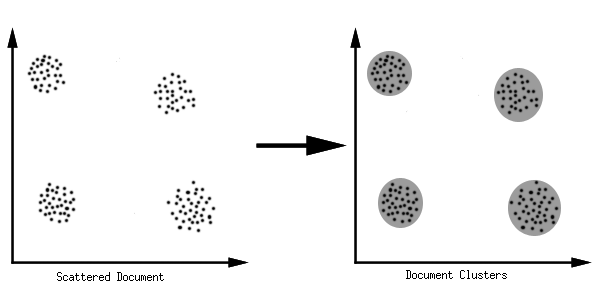
\includegraphics[width=0.9\textwidth]{figures/clustering}
  \caption{Clustering Process}
  \label{fig:clustering}
\end{figure}

In Figure \ref{fig:clustering} we can easily identify the 4 clusters into which the data can be divided; the similarity
criterion is \textit{distance}: two or more objects belong to the same cluster\index{Cluster} if they are ``close" according to a
given distance (in this case geometrical distance). This is called \textit{distance-based clustering}.
Another kind of clustering is \textit{conceptual clustering}: two or more objects belong to the same cluster
if this one defines a concept common to all that objects. In other words, objects are grouped according
to their fit to descriptive concepts, not according to simple similarity measures.

The main goal of clustering is to determine the intrinsic grouping in a given set of unlabeled data.
But there is no such factors to decide what constitutes a good clustering. It can be shown that there is no
absolute ``best" criterion which would be independent of the final aim of the clustering. Consequently, it is the user
which must supply this criterion, in such a way that the result of the clustering will suit their needs.
For instance, we could be interested in finding representatives for homogeneous groups (data reduction),
in finding ``natural clusters"\index{Natural Clusters} and describe their unknown properties (``natural" data types),
in finding useful and suitable groupings (``useful" data classes) or in finding unusual data objects (outlier detection).

\subsection{Applications}
Clustering algorithms can be applied in a very wide range of fields. In \textit{Marketing}\index{Marketing} we can use clustering
to find groups of customers with similar behavior from a large database of customers data containing their properties
and past buying records. In \textit{Biology}\index{Biology} we can classify plants and animals by their given feature sets. Book
ordering and sorting can be a good application of clustering in the \textit{Libraries}\index{Libraries}. \textit{Insurance}\index{Insurance} companies
use clustering for identifying groups of insurance policy holders with a high average claim cost.
Recently urban developers are using clustering methods for identifying groups
of houses according to their house type, value and geographical location in \textit{city-planning}\index{Uraban Planning}. To identify
dangerous zones of earthquake we can observe earthquake epicenters by using clustering algorithms on. These days
clustering algorithms are mostly used in \textit{WWW}\index{World Wide Web} for document classification;
clustering weblog data to discover groups of similar access patterns.

\subsection{Requirements}
The main requirements that a clustering algorithm should satisfy are:
\begin{itemize}
\item \textbf{Scalability} : We need highly scalable clustering algorithms to deal with large databases.
\item \textbf{Ability to deal with different kinds of attributes} : Algorithms should be capable to be applied on any kind of data such as interval-based (numerical) data, categorical, and binary data.
\item \textbf{Discovery of clusters with attribute shape} : The clustering algorithm should be capable of detecting clusters of arbitrary shape. They should not be bounded to only distance measures that tend to find spherical cluster of small sizes.
\item \textbf{High dimensionality} : The clustering algorithm should not only be able to handle low-dimensional data but also the high dimensional space.
\item \textbf{Ability to deal with noisy data} : Databases contain noisy, missing or erroneous data. Some algorithms are sensitive to such data and may lead to poor quality clusters.
\item \textbf{Interpretability} : The clustering results should be interpretable, comprehensible, and usable.
\end{itemize}

\subsection{Problems}
There are a number of problems with clustering. Among them:
\begin{itemize}
\item Current clustering techniques do not address all the requirements adequately (and concurrently);
\item Dealing with large number of dimensions and large number of data items can be problematic because of time complexity;
\item The effectiveness of the method depends on the definition of “distance” (for distance-based clustering);
\item If an obvious distance measure doesn’t exist we must “define” it, which is not always easy, especially in multi-dimensional spaces;
\item The result of the clustering algorithm (that in many cases can be arbitrary itself) can be interpreted in different ways.
\end{itemize}

\subsection{Classification}
Clustering algorithms may be classified as listed below:
\begin{itemize}
\item \textbf{Hierarchical Clustering} : Hierarchical clustering,\index{Hierarchical Clustering} is based on the core idea of objects being more
related to nearby objects than to objects farther away. These algorithms connect ``objects" to form ``clusters"
based on their distance. A cluster can be described largely by the maximum distance needed to connect parts of
the cluster. At different distances, different clusters will form, which can be represented using a \textit{dendrogram},
which explains where the common name ``Hierarchical Clustering" comes from: these algorithms do not provide a
single partitioning of the data set, but instead provide an extensive hierarchy of clusters that merge with each
other at certain distances. In a dendrogram\index{Dendrogram}, the Y-axis marks the distance at which the clusters merge, while the
objects are placed along the X-axis such that the clusters don't mix.

Connectivity based clustering\index{Connectivity Based Clustering} is a whole family of methods that differ by the way distances are computed.
Apart from the usual choice of \textit{distance functions}\index{Distance Functions}, the user also needs to decide on the linkage criterion
(since a cluster consists of multiple objects, there are multiple candidates to compute the distance to) to use.
Popular choices are known as \textit{single-linkage clustering}\index{Single Linkage Clustering} (the minimum of object distances),
\textit{complete linkage clustering}\index{Complete Linkage Clustering} (the maximum of object distances) or UPGMA (``Unweighted Pair Group Method with
Arithmetic Mean"\index{UPGMA}, also known as average linkage clustering)\index{Average Linkage Clustering}. Furthermore, hierarchical clustering can be
agglomerative (starting with single elements and aggregating them into clusters) or divisive
(starting with the complete data set and dividing it into partitions).

These methods will not produce a unique partitioning of the data set, but a hierarchy from which the user still
needs to choose appropriate clusters. They are not very robust towards outliers, which will either show up as
additional clusters or even cause other clusters to merge (known as ``chaining phenomenon", in particular with
single-linkage clustering). In the general case, the complexity is $O(n^{3})$ for agglomerative clustering and
$O(2^{n-1})$ for \textit{divisive clustering}\index{Divisive Clustering}, which makes them too slow for large data sets. For some special cases,
optimal efficient methods (of complexity $O(n^{2})$ are known as single-linkage and complete-linkage clustering.
In the \textit{data mining}\index{Data Mining} community these methods are recognized as a theoretical foundation of cluster analysis,
but often considered obsolete. They did however provide inspiration for many later methods such as density based
clustering.


\item \textbf{Centroid-based Clustering} : In centroid-based clustering\index{Centroid Based Clustering}, clusters are represented by a central vector,
which may not necessarily be a member of the data set. When the number of clusters is fixed to k, k-means clustering
gives a formal definition as an optimization problem: find the k cluster centers and assign the objects to the nearest
cluster center, such that the squared distances from the cluster are minimized.

The optimization problem\index{Optimization Problem} itself is known to be NP-hard, and thus the common approach is to search only for approximate
solutions. A particularly well known approximative method is Lloyd's algorithm, often actually referred to as
``$K$-means algorithm". It does however only find a local optimum, and is commonly run multiple times with different
random initializations. Variations of $K$-means\index{K-means} often include such optimizations as choosing the best of multiple runs,
but also restricting the centroids to members of the data set (k-medoids)\index{K-medoids}, choosing medians (k-medians clustering),
choosing the initial centers less randomly (k-means++) or allowing a fuzzy cluster assignment (fuzzy c-means)\index{fuzzy C-means}.

Most k-means-type algorithms require the number of clusters - k to be specified in advance, which is considered
to be one of the biggest drawbacks of these algorithms. Furthermore, the algorithms prefer clusters of approximately
similar size, as they will always assign an object to the nearest centroid. This often leads to incorrectly cut
borders of clusters (which is not surprising since the algorithm optimizes cluster centers, not cluster borders).

\item \textbf{Distribution-based clustering} :\index{Distribution Based Clustering} The clustering model most closely related to statistics is based
on distribution models. Clusters can then easily be defined as objects belonging most likely to the same distribution.
A convenient property of this approach is that this closely resembles the way artificial data sets are generated:
by sampling random objects from a distribution.

While the theoretical foundation of these methods is excellent, they suffer from one key problem known as overfitting\index{Overfitting},
unless constraints are put on the model complexity. A more complex model will usually be able to explain the data better,
which makes choosing the appropriate model complexity inherently difficult.

One prominent method is known as Gaussian mixture models\index{Gaussian Mixture Models} (using the expectation-maximization algorithm). Here,
the data set is usually modelled with a fixed (to avoid overfitting) number of Gaussian distributions that are
initialized randomly and whose parameters are iteratively optimized to better fit the data set. This will converge
to a local optimum, so multiple runs may produce different results. In order to obtain a hard clustering, objects
are often then assigned to the Gaussian distribution they most likely belong to; for soft clusterings, this is not
necessary.

Distribution-based clustering produces complex models for clusters that can capture correlation and dependence
between attributes. However, these algorithms put an extra burden on the user: for many real data sets, there may
be no concisely defined mathematical model (e.g. assuming Gaussian distributions is a rather strong assumption
on the data).

\item \textbf{Density-based Clustering} : In density-based clustering\index{Density Based Clustering}, clusters are defined as areas of higher density
than the remainder of the data set. Objects in these sparse areas that are required to separate clusters are usually
considered to be noise and border points.

The most popular density based clustering method is DBSCAN. In contrast to many newer methods, it features a well-defined
cluster model called ``density-reachability". Similar to linkage based clustering, it is based on connecting points within
certain distance thresholds. However, it only connects points that satisfy a density criterion, in the original variant
defined as a minimum number of other objects within this radius. A cluster consists of all density connected objects
(which can form a cluster of an arbitrary shape, in contrast to many other methods) plus all objects that are within
these objects' range. Another interesting property of DBSCAN is that its complexity is fairly low it requires a linear
number of range queries on the database - and that it will discover essentially the same results (it is deterministic
for core and noise points, but not for border points) in each run, therefore there is no need to run it multiple times.
OPTICS is a generalization of DBSCAN that removes the need to choose an appropriate value for the range parameter ${\varepsilon}$,
and produces a hierarchical result related to that of linkage clustering. DeLi-Clu, Density-Link-Clustering\index{Density Link Clustering} combines ideas
from single-linkage clustering and OPTICS, eliminating the ${\varepsilon}$ parameter entirely and offering performance improvements
over OPTICS by using an R-tree index.

The key drawback of DBSCAN\index{DBSCAN} and OPTICS\index{OPTICS} is that they expect some kind of density drop to detect cluster borders.
On data sets with, for example, overlapping Gaussian distributions a common use case in artificial data the
cluster borders produced by these algorithms will often look arbitrary, because the cluster density decreases
continuously. On a data set consisting of mixtures of Gaussians, these algorithms are nearly always outperformed
by methods such as EM clustering that are able to precisely model this kind of data.

Mean-shift is a clustering approach where each object is moved to the densest area in its vicinity, based on kernel
density estimation. Eventually, objects converge to local maxima\index{Local Maxima} of density. Similar to k-means clustering, these
``density attractors"\index{Density Attractors} can serve as representatives for the data set, but mean-shift can detect arbitrary-shaped
clusters similar to DBSCAN. Due to the expensive iterative procedure and density estimation, mean-shift\index{Mean Shift} is usually
slower than DBSCAN or k-Means. Besides that, the applicability of the mean-shift algorithm to multidimensional data
is hindered by the unsmooth behaviour of the kernel density estimate, which results in over-fragmentation of cluster
tails.
\end{itemize}

\section{Literature Survey}

\subsection{Values of K specified within a range or set}
The  performance  of  a  clustering  algorithm  may  be
affected by the chosen value of K. Therefore, instead
of using a single predefined K, a set of values might
be   adopted.   It   is   important   for   the   number   of
values  considered  to  be  reasonably  large,  to  reflect
the  specific  characteristics  of  the  data  sets.  At  the
same  time,  the  selected  values  have  to  be  significantly
smaller  than  the  number  of  objects  in  the
data sets, which is the main motivation for performing data clustering.

Reported studies~\cite{han00, daoud95, daoud96, ranka98, bilmes97, bengio95}
on K-means clustering and
its  applications  usually  do  not  contain  any  explanation
or  justification  for  selecting  particular  values for K.
First,  a  number  of  researchers~\cite{bilmes97, bengio95} used  only  one  or  two  values  for K.
Second, several  other  researchers~\cite{han00, daoud96} utilized relatively  large K
values  compared  with  the  number of  objects.  These  two  actions  contravene
the  above mentioned  guidelines  for  selecting K. Therefore,the
clustering  results  do  not  always  correctly  represent
the performance of the tested algorithms.

In  general,  the  performance  of  any  new  version
of the K-means algorithm could be verified by com-
paring  it  with  its  predecessors  on  the  same  criteria.
In   particular,   the   sum   of   cluster   distortions   is
usually  employed  as  such  a  performance  indicator.~\cite{daoud96, bengio95}
Thus, the comparison is considered fair  because  the  same  model and  criterion  are  used
for the performance analysis.

\subsection{Values of K specified by the user}
The K-means  algorithm  implementation  in  many
data-mining   or   data   analysis   software   packages~\cite{hall02}
requires the number of clusters to be specified
by  the  user.  To  find  a  satisfactory  clustering
result,  usually,  a  number  of  iterations  are  needed
where the user executes the algorithm with different
values  of K.  The  validity  of  the  clustering  result  is
assessed  only  visually  without  applying  any  formal
performance   measures.   With   this   approach,   it   is
difficult  for  users  to  evaluate  the  clustering  result
for multi-dimensional data sets.

\subsection{Values of K determined in a later processing step}
When K-means clustering is used as a pre-processing
tool,  the  number  of  clusters  is  determined  by  the
specific requirements of the main processing algorithm.~\cite{hansen96}
No  attention  is  paid  to  the  effect  of
the  clustering  results  on  the  performance  of  this
algorithm. In such applications, the K-means
algorithm  is  employed  just  as  a  'black  box'  without
validation of the clustering result.

\subsection{Values of K equated to the number of generators}
Synthetic   data   sets,   which   are   used   for   testing
algorithms,  are  often  created  by  a  set  of  normal  or
uniform   distribution   generators.   Then,   clustering
algorithms  are  applied  to  those  data  sets  with  the
number of clusters equated to the number of generators.
It  is  assumed  that  any  resultant  cluster  will
cover  all  objects  created  by  a  particular  generator.
Thus,  the  clustering  performance  is  judged  on  the
basis  of  the  difference  between  objects  covered  by
a  cluster  and  those  created  by  the  corresponding
generator.  Such  a  difference  can  be  measured  by
simply   counting   objects   or   calculating   the
information gain.~\cite{bradly98}

Unfortunately,  this  method  of  selecting K cannot
be  applied  to  practical  problems.  The  data  distribution
in  practical  problems  is  unknown  and  also
the number of generators cannot be specified.

\subsection{Values of K determined by statistical measures}
There  are  several  statistical  measures  available  for
selecting K. These measures are often applied in combination
with   probabilistic   clustering   approaches.
They are calculated with certain assumptions
about  the  underlying  distribution  of  the  data.  The
Bayesian   information   criterion\index{Bayesian Information Criterion}   or   Akeike’s   information~\cite{ishioka00}
criterion  is  calculated  on  data  sets
which  are  constructed  by  a  set  of  Gaussian  distributions.
The  measures  applied  by  Hardy  are
based  on  the  assumption  that  the  data  set  fits  the
Poisson distribution. Monte Carlo techniques,\index{Monte Carlo}
which  are  associated  with  the null  hypothesis\index{Null Hypothesis},  are
used for assessing the clustering results and also for
determining the number of clusters.

\subsection{Values of K determined through visualization}
Visual  verification  is  applied  widely  because  of  its
simplicity and explanation possibilities. Visual
examples  are  often  used  to  illustrate  the  drawbacks
of an algorithm or to present the expected clustering
results.~\cite{bilmes97}

The    assessment    of    a    clustering    result    using
visualization  techniques  depends  heavily  on  their
implicit  nature.  The  clustering  models  utilized  by
some  clustering  methods  may  not  be  appropriate
for   particular   data   sets. The  application  of
visualization  techniques  implies  a  data  distribution
continuity  in  the  expected  clusters.  If  the K-means
approach  is  applied  to  such  data  sets,  there  is  not
any    cluster    that    satisfies   the K-means   clustering
model  and  at  the  same  time  corresponds  to  a
particular   object   grouping   in   the   illustrated   data
sets.  Therefore,  the K-means  algorithm  cannot  produce
the  expected  clustering  results.  This  suggests
that  the K-means  approach  is  unsuitable  for  such
data sets.

\section{Objective}
Partitioning methods or Centroid-base Clustering algorithms, such as $K$-means clustering require the users to specify
the number of clusters to be generated. One fundamental question is: If the data is clusterable, then how to choose the
right number of expected clusters $K$? Unfortunately, there is no definitive answer to this question. The optimal
clustering is somehow subjective and depend on the method used for measuring similarities and the parameters used for
partitioning.

In this work, our prime objectives are:

\begin{itemize}
\item Describing different methods of determining the optimal number of clusters for $K$-means clustering.
\item These methods include direct methods and statistical testing methods. Direct methods consists of
optimizing a criterion, such as the within cluster sums of squares or the average silhouette. Statistical
testing methods consists of comparing evidence against null hypothesis. An example is the gap statistic.
\item We'll apply these methods on various data sets and find the optimal number of clusters for $K$-means clustering.
\item Finally we'll compare performance among these methods on the basis of determining number of clusters for
different data sets.
\end{itemize}

\section{Thesis Organization}
In Chapter One, we try to give a general overview about what is machine learning, clustering,
why clustering is so important and what are the factors behind determining number of clusters.
In Chapter Two, we will discuss the idea behind determining number of clusters of a dataset and
how it affects the output of $K$-means algorithm.
In Chapter Three, we will describe different methods for selecting number of clusters and there approach,
algorithms.
In Chapter Four, we want to show experimental result of our reviewed methods algorithm and output.
Then we'll compare the output with the original output.
In Chapter Five, we put a discussion about the future of this work, where it can give promising
result and how it can be improved further.

\endinput


% Chapter-2 Background
\chapter{Background}\label{background}

\section{Introduction}
Machine learning\index{Machine Learning} is the subfield of computer science that gives computers the ability to learn
without being explicitly programmed. Evolved from the study of pattern recognition and computational
learning theory in artificial intelligence, machine learning explores the study and
construction of algorithms that can learn from and make predictions on data such algorithms
overcome following strictly static program instructions by making data driven predictions or
decisions, through building a model from sample inputs. Machine learning is employed in a
range of computing tasks where designing and programming explicit algorithms is infeasible;
example applications include spam filtering, detection of network intruders or malicious insiders
working towards a data breach, optical character recognition (OCR)\index{OCR}, search engines and
computer vision\index{Computer Vision}.\\

Tom M. Mitchell~\cite{Michalski2013ml} provided a widely quoted, more formal definition:

``A computer program is said to learn from experience E with respect to some class
of tasks T and performance measure P if its performance at tasks in T, as measured
by P, improves with experience E."

Machine learning tasks are typically classified into three broad categories, depending on the
nature of the learning ``signal" or ``feedback" available to a learning system.

\subsubsection{Supervised Learning}
Supervised learning\index{Supervised Learning} is where you have input variables ($x$) and an output variable ($Y$) and
you use an algorithm to learn the mapping function from the input to the output. Exact functon
may be as $Y$ = $f(X)$. The goal is to approximate the mapping function so well that when you
have new input data ($x$) that you can predict the output variables ($Y$) for that data.

It is called supervised learning because the process of an algorithm learning from the training
dataset can be thought of as a teacher supervising the learning process. We know the correct
answers, the algorithm iteratively makes predictions on the training data and is corrected by the
teacher. Learning stops when the algorithm achieves an acceptable level of performance. Supervised
learning problems can be further grouped into regression and classification problems.

\begin{itemize}
\item \textbf{Classification} : A classification\index{Classification Problem} problem is when the output variable is a category, such as
``red" or ``blue" or ``disease" and ``no disease".
\item \textbf{Regression} : A regression\index{Regression Problem} problem is when the output variable is a real value, such as
``dollars" or ``weight".\\
\end{itemize}

\subsubsection{Unsupervised Learning}
No labels are given to the learning algorithm\index{Unsupervised Learning}, leaving it on its own to find structure in its
input. Unsupervised learning can be a goal in itself (discovering hidden patterns in data) or a
means towards an end (feature learning).Unsupervised learning is where you only have input
data $(X)$ and no corresponding output variables.

The goal for unsupervised learning is to model the underlying structure or distribution in the
data in order to learn more about the data.These are called unsupervised learning because unlike
supervised learning above there is no correct answers and there is no teacher. Algorithms are left
to their own devises to discover and present the interesting structure in the data.Unsupervised
learning problems can be further grouped into clustering and association problems.

\begin{itemize}
\item \textbf{Clustering} : A clustering problem\index{Clustering Problem} is where you want to discover the inherent groupings
in the data, such as grouping customers by purchasing behavior.
\item \textbf{Association} : An association\index{Association Problem} rule learning problem is where you want to discover rules
that describe large portions of your data, such as people that buy X also tend to buy Y.\\
\end{itemize}

\section{A Deep Dive into Cluster Analysis}
Cluster analysis\index{Cluster Analysis} groups data objects based only on information found in the
data that describes the objects and their relationships.  The goal is that the
objects within a group be similar (or related) to one another and different from
(or unrelated to) the objects in other groups.  The greater the similarity (or
homogeneity) within a group and the greater the difference between groups,
the better or more distinct the clustering.

Cluster analysis is related to other techniques that are used to divide data
objects into groups.  For instance, clustering can be regarded as a form of
classification in that it creates a labeling of objects with class (cluster) labels.
However, it derives these labels only from the data. In contrast, classification
in the sense of our previous section is \textbf{supervised classification}\index{Supervised Classification}; i.e.,
new, unlabeled objects are assigned a class label using a model developed from objects with
known class labels. For this reason, cluster analysis is sometimes referred to as
\textbf{unsupervised classification}\index{Unsupervised Classification}. When the term classification is used
without any qualification within data mining, it typically refers to supervised
classification.

\subsection{Centroid Based Cluster}
A cluster is a set of objects in which each object is closer
(more similar) to the center that defines the cluster than to the centers
of any other cluster\index{Centroid Based Clustering}.  For data with continuous attributes, the prototype of a
cluster is often a centroid, i.e., the average (mean) of all the points in the cluster.
When a centroid is not meaningful, such as when the data has categorical
attributes, the prototype is often a medoid, i.e., the most representative point
of a cluster.  For many types of data, the centroid can be regarded as the
most central point. One of the most popular centroid-based algorithm is $K$-means. Let's
have a look on to the details about $K$-means algorithm.

\subsection{$K$-means}
Centroid-based clustering techniques create a one-level partitioning of the
data objects.  There are a number of such techniques, but two of the most
prominent are $K$-means and $K$-medoid. $K$-means defines a prototype in terms
of a centroid, which is usually the mean of a group of points, and is typically
applied to objects in a continuous $n$ dimensional space.  $K$-medoid defines a
prototype in terms of a medoid, which is the most representative point for a
group of points, and can be applied to a wide range of data since it requires
only a proximity measure for a pair of objects. While a centroid almost never
corresponds to an actual data point, a medoid, by its definition, must be an
actual data point.  In this subsection, we will focus solely on $K$-means, which is
one of the oldest and most widely used clustering algorithms and our objective is based on this algorithm.

\subsection{The Basic $K$-means Algorithm}
The $K$-means clustering technique is simple, and we begin with a description
of the basic algorithm. We first choose $K$ initial centroids, where $K$ is a user-specified
parameter, namely, the number of clusters desired.  Each point is
then assigned to the closest centroid, and each collection of points assigned to
a centroid is a cluster. The centroid of each cluster is then updated based on
the points assigned to the cluster. We repeat the assignment and update steps
until no point changes clusters, or equivalently, until the centroids remain the
same.

K-means is formally described by Algorithm~\ref{alg0}

\begin{algorithm}
  \caption{Basic $K$-means algorithm.}
  \label{alg0}
  \begin{algorithmic}
    \input{algorithms/kmeans.alg}
  \end{algorithmic}
\end{algorithm}

\subsection{Assigning Points to the Closest Centroid}
To assign a point to the closest centroid, we need a proximity measure that
quantifies the notion of ``closest" for the specific data under consideration.
Euclidean (L2) distance\index{Euclidean Distance} is often used for data points in Euclidean space, while
cosine similarity is more appropriate for documents.  However, there may be
several types of proximity measures that are appropriate for a given type of
data. For example, Manhattan (L1) distance\index{Manhattan Distance} can be used for Euclidean data,
while the Jaccard measure is often employed for documents.

Usually, the similarity measures used for $K$-means are relatively simple
since the algorithm repeatedly calculates the similarity of each point to each
centroid. In some cases, however, such as when the data is in low-dimensional
Euclidean space, it is possible to avoid computing many of the similarities,
thus significantly speeding up the $K$-means algorithm.   Bisecting $K$-means
is another approach that speeds up $K$-means by reducing the number of similarities computed.

\subsection{Centroids and Objective Functions}
Step 4 of the $K$-means algorithm was stated rather generally as ``recompute
the centroid of each cluster," since the centroid can vary, depending on the
proximity measure for the data and the goal of the clustering.  The goal of
the clustering is typically expressed by an objective function that depends on
the proximities of the points to one another or to the cluster centroids; e.g.,
minimize the squared distance of each point to its closest centroid. However,
the key point is this: once we have
specified a proximity measure and an objective function, the centroid that we
should choose can often be determined mathematically.

\subsection{Data in Euclidean Space}
Consider data whose proximity measure is Euclidean distance.
For our objective function, which measures the quality of a
clustering, we use the sum of the squared error (SSE), which is also known
as scatter.  In other words, we calculate the error of each data point, i.e., its
Euclidean distance to the closest centroid, and then compute the total sum
of the squared errors.  Given two different sets of clusters that are produced
by two different runs of $K$-means, we prefer the one with the smallest squared
error since this means that the prototypes (centroids) of this clustering are
a better representation of the points in their cluster.\\

\hangindent=0.5cm
$SSE$ = $\sum_{i=1}^{K}$ $\sum_{x \epsilon C_i}$ $dist(C_i, x)^2$
\\\\Where,
$x$ = An object.\\
$C_i$ = The i\'th cluster.\\
$c_i$ = The centroid of cluster $C_i$.\\
$c$ = The centroid of all points.\\
$m_i$ = The number of objects in the i\'th cluster.\\
$m$ = The number of objects in the dataset.\\
$K$ = The number of clusters.\\
$dist$ = Standard Euclidean distance between two objects in Euclidean Space.\\

\subsection{Choosing Initial Centroids}
When random initialization of centroids is used, different runs of $K$-means
typically produce different total $SSE$s. Choosing the proper initial centroids
is the key step of the basic $K$-means procedure.  A common approach is to choose
the initial centroids randomly, but the resulting clusters are often poor.

An optimal clustering will be obtained as long as two initial
centroids fall anywhere in a pair of clusters, since the centroids will redistribute
themselves,  one to each cluster. Unfortunately,  as the number of clusters
becomes larger, it is increasingly likely that at least one pair of clusters will
have only one initial centroid. In this case,
because the pairs of clusters are farther apart than clusters within a pair, the
K-means algorithm will not redistribute the centroids between pairs of clusters,
and thus, only a local minimum will be achieved.

Because of the problems with using randomly selected initial centroids,
which even repeated runs may not overcome, other techniques are often employed
for initialization.  One effective approach is to take a sample of points
and cluster them using a hierarchical clustering technique. $K$ clusters are extracted
from the hierarchical clustering, and the centroids of those clusters are
used as the initial centroids. This approach often works well, but is practical
only if the sample is relatively small, e.g., a few hundred to a few thousand
(because hierarchical clustering is expensive), and $K$ is relatively small compared
to the sample size.

\subsection{Updating Centroids Incrementally}
Instead of updating cluster centroids after all points have been assigned to a
cluster, the centroids can be updated incrementally, after each assignment of
a point to a cluster.  Notice that this requires either zero or two updates to
cluster centroids at each step, since a point either moves to a new cluster (two
updates) or stays in its current cluster (zero updates).  Using an incremental
update strategy guarantees that empty clusters are not produced since all
clusters start with a single point, and if a cluster ever has only one point, then
that point will always be reassigned to the same cluster.

In addition, if incremental updating is used, the relative weight of the point
being added may be adjusted; e.g., the weight of points is often decreased as
the clustering proceeds.  While this can result in better accuracy and faster
convergence, it can be difficult to make a good choice for the relative weight,
especially in a wide variety of situations.  These update issues are similar to
those involved in updating weights for artificial neural networks.

Yet another benefit of incremental updates has to do with using objectives
other than ``minimize $SSE$."\index{SSE} Suppose that we are given an arbitrary objective
function to measure the goodness of a set of clusters.  When we process an
individual point, we can compute the value of the objective function for each
possible cluster assignment, and then choose the one that optimizes the objective.

On the negative side, updating centroids incrementally introduces an order dependency.
In other words, the clusters produced may depend on the
order in which the points are processed.  Although this can be addressed by
randomizing the order in which the points are processed, the basic $K$-means
approach of updating the centroids after all points have been assigned to clusters
has no order dependency.  Also, incremental updates are slightly more
expensive.   However,  $K$-means converges rather quickly,  and therefore,  the
number of points switching clusters quickly becomes relatively small.

\endinput


% Citation examples
\chapter{Citation Examples}\label{ch:citations}

In this chapter we show how we can cite the references.


\section{See the Citations}
\label{sec:cite}

As discussed by authors
in~\cite{akbar2006solving,karim2015comograd,alam2012diversity} we can
further show how this affects
us. Moreover~\cite{kaykobad1987nonnegative,kaykobad1985positive,kaykobad19983,MCNC,guo2001floorplanning,holland1975as,aickelin2005artificial,al2010artificial}
can be examples for the previous works. Among
these~\cite{aickelin2005artificial,faruque2016modelling,durocher2015graphs,rahman2016absent,hashem2013countering,farhad2016mapping,malek2016balanced}
are the prominent ones. Also you can take a look
at~\cite{bashir2016learning,uddin2014citizen,kamal2016boosting,haque2013constructing,mukta2016identifying,ali2016spatial,islam2009new,al2010stable}.


\endinput





% Another chapter
\chapter{Another Chapter}\label{anotherchapter}


\section{A Section}
Some text.
\subsection{This is a Subsection}
And some more.
\subsubsection{This is a Subsubsection}
Yet some more.

\section{And Another Section}

Here are some dummy texts.

Lorem ipsum dolor sit amet, consectetur adipiscing elit. Cras et
ultricies massa. Nulla a sapien lobortis, dignissim nibh in, aliquet
mauris. Integer at dictum metus. Quisque in tortor congue ipsum
ultricies tristique. Maecenas ut tortor dapibus, sagittis enim at,
tincidunt massa. Ut sollicitudin sagittis ipsum, ac tincidunt quam
gravida ac. Nullam quis faucibus purus. Aliquam vel pretium
turpis. Aliquam a quam non ex interdum sagittis id vitae quam. Nullam
sodales ligula malesuada maximus consequat. Proin a justo eget lacus
vulputate maximus luctus vitae enim. Aliquam libero turpis, pharetra a
tincidunt ac, pulvinar sit amet urna. Pellentesque eget rutrum diam,
in faucibus sapien. Aenean sit amet est felis. Aliquam dolor eros,
porttitor quis volutpat eget, posuere a ligula. Proin id velit ac
lorem finibus pellentesque.

Maecenas vitae interdum mi. Aenean commodo nisl massa, at pharetra
libero cursus vitae. In hac habitasse platea dictumst. Suspendisse
iaculis euismod dui, et cursus diam. Nullam euismod, est ut dapibus
condimentum, lorem eros suscipit risus, sit amet hendrerit justo
tortor nec lorem. Morbi et mi eget erat bibendum porta. Ut tristique
ultricies commodo. Nullam iaculis ligula sed lacinia ornare.

Sed ultricies cursus nisi at vestibulum. Aenean laoreet viverra
efficitur. Ut eget sapien lorem. Mauris malesuada, augue in pulvinar
consectetur, ex tortor tristique ligula, sit amet faucibus metus
lectus interdum nisl. Nam eget turpis vitae ligula pulvinar bibendum a
ut ipsum. Mauris fringilla lacinia malesuada. Fusce id orci
velit. Donec tristique rhoncus urna, a hendrerit arcu vehicula
imperdiet. Integer tristique erat at gravida condimentum. Sed ornare
cursus quam, eget tincidunt enim bibendum sed. Aliquam elementum
ligula scelerisque leo sagittis, quis convallis elit dictum. Donec sit
amet orci aliquam, ultricies sapien nec, gravida nisi. Etiam et
pulvinar diam, et pellentesque arcu. Nulla interdum metus sed aliquet
consequat.

Proin in mi id nulla interdum aliquet ac quis arcu. Duis blandit
sapien commodo turpis hendrerit pharetra. Phasellus sit amet justo
orci. Proin mattis nisl dictum viverra fringilla. Interdum et
malesuada fames ac ante ipsum primis in faucibus. Curabitur facilisis
euismod augue vestibulum tincidunt. Nullam nulla quam, volutpat vitae
efficitur eget, porta sit amet nunc. Phasellus pharetra est eget urna
ornare volutpat. Aenean ultrices, libero eget porttitor fringilla,
purus tortor accumsan neque, sit amet viverra felis tortor eget
justo. Nunc id metus a purus tempus euismod condimentum non lacus. Nam
vitae diam aliquam, facilisis diam quis, pharetra nunc. Nulla eget
vestibulum tellus, ut cursus tellus. Vestibulum euismod pellentesque
sodales.

Maecenas at mi interdum, faucibus lorem sed, hendrerit nisi. In vitae
augue consequat diam commodo porta sit amet eu purus. Mauris mattis
condimentum feugiat. Nulla commodo molestie risus vitae maximus. Proin
hendrerit neque malesuada urna laoreet convallis. Etiam a diam
pulvinar, auctor sem ac, hendrerit risus. Ut urna urna, venenatis ac
tellus non, scelerisque tristique ligula. Vestibulum sollicitudin vel
leo malesuada accumsan. Donec sit amet erat diam. Vestibulum ante
ipsum primis in faucibus orci luctus et ultrices posuere cubilia
Curae; Vivamus odio dui, scelerisque et lorem egestas, posuere
ullamcorper nunc. Integer varius nunc nec velit tincidunt
commodo. Mauris rhoncus ultrices sapien non suscipit.


Lorem ipsum dolor sit amet, consectetur adipiscing elit. Cras et
ultricies massa. Nulla a sapien lobortis, dignissim nibh in, aliquet
mauris. Integer at dictum metus. Quisque in tortor congue ipsum
ultricies tristique. Maecenas ut tortor dapibus, sagittis enim at,
tincidunt massa. Ut sollicitudin sagittis ipsum, ac tincidunt quam
gravida ac. Nullam quis faucibus purus. Aliquam vel pretium
turpis. Aliquam a quam non ex interdum sagittis id vitae quam. Nullam
sodales ligula malesuada maximus consequat. Proin a justo eget lacus
vulputate maximus luctus vitae enim. Aliquam libero turpis, pharetra a
tincidunt ac, pulvinar sit amet urna. Pellentesque eget rutrum diam,
in faucibus sapien. Aenean sit amet est felis. Aliquam dolor eros,
porttitor quis volutpat eget, posuere a ligula. Proin id velit ac
lorem finibus pellentesque.

Maecenas vitae interdum mi. Aenean commodo nisl massa, at pharetra
libero cursus vitae. In hac habitasse platea dictumst. Suspendisse
iaculis euismod dui, et cursus diam. Nullam euismod, est ut dapibus
condimentum, lorem eros suscipit risus, sit amet hendrerit justo
tortor nec lorem. Morbi et mi eget erat bibendum porta. Ut tristique
ultricies commodo. Nullam iaculis ligula sed lacinia ornare.

Sed ultricies cursus nisi at vestibulum. Aenean laoreet viverra
efficitur. Ut eget sapien lorem. Mauris malesuada, augue in pulvinar
consectetur, ex tortor tristique ligula, sit amet faucibus metus
lectus interdum nisl. Nam eget turpis vitae ligula pulvinar bibendum a
ut ipsum. Mauris fringilla lacinia malesuada. Fusce id orci
velit. Donec tristique rhoncus urna, a hendrerit arcu vehicula
imperdiet. Integer tristique erat at gravida condimentum. Sed ornare
cursus quam, eget tincidunt enim bibendum sed. Aliquam elementum
ligula scelerisque leo sagittis, quis convallis elit dictum. Donec sit
amet orci aliquam, ultricies sapien nec, gravida nisi. Etiam et
pulvinar diam, et pellentesque arcu. Nulla interdum metus sed aliquet
consequat.

Proin in mi id nulla interdum aliquet ac quis arcu. Duis blandit
sapien commodo turpis hendrerit pharetra. Phasellus sit amet justo
orci. Proin mattis nisl dictum viverra fringilla. Interdum et
malesuada fames ac ante ipsum primis in faucibus. Curabitur facilisis
euismod augue vestibulum tincidunt. Nullam nulla quam, volutpat vitae
efficitur eget, porta sit amet nunc. Phasellus pharetra est eget urna
ornare volutpat. Aenean ultrices, libero eget porttitor fringilla,
purus tortor accumsan neque, sit amet viverra felis tortor eget
justo. Nunc id metus a purus tempus euismod condimentum non lacus. Nam
vitae diam aliquam, facilisis diam quis, pharetra nunc. Nulla eget
vestibulum tellus, ut cursus tellus. Vestibulum euismod pellentesque
sodales.

Maecenas at mi interdum, faucibus lorem sed, hendrerit nisi. In vitae
augue consequat diam commodo porta sit amet eu purus. Mauris mattis
condimentum feugiat. Nulla commodo molestie risus vitae maximus. Proin
hendrerit neque malesuada urna laoreet convallis. Etiam a diam
pulvinar, auctor sem ac, hendrerit risus. Ut urna urna, venenatis ac
tellus non, scelerisque tristique ligula. Vestibulum sollicitudin vel
leo malesuada accumsan. Donec sit amet erat diam. Vestibulum ante
ipsum primis in faucibus orci luctus et ultrices posuere cubilia
Curae; Vivamus odio dui, scelerisque et lorem egestas, posuere
ullamcorper nunc. Integer varius nunc nec velit tincidunt
commodo. Mauris rhoncus ultrices sapien non suscipit.


\endinput

% Chapter showing example of index creation
\chapter{Index Creation}
\section{BUET}
Bangladesh University of Engineering and Technology, abbreviated as
BUET\index{BUET}, is one of the most prestigious institutions for
higher studies in the country. About 5500 students are pursuing
undergraduate\index{BUET!undergraduate} and
postgraduate\index{BUET!postgraduate} studies in engineering,
architecture, planning and science in this institution. At present,
BUET has sixteen teaching departments under five faculties and it has
three institutes. Every year the intake of undergraduate students is
around 900, while the intake of graduate students in Master's and PhD
programs is around 1000. A total of about five hundred teachers are
teaching in these departments and institutes. There are additional
teaching posts like Dr.\ Rashid Professor, Professor Emeritus and
Supernumerary Professors.
 
\section{Campus}
The BUET campus is in the heart of Dhaka\index{Dhaka} --- the capital
city of Bangladesh. It has a compact campus with halls of residence
within walking distances of the academic buildings. The physical
expansion of the University over the last three decades has been
impressive with construction of new academic buildings,
auditorium\index{BUET!auditorium} complex, halls of residence, etc.
 
\section{History}\index{BUET!History}
BUET is the oldest institution for the study of Engineering and
Architecture in Bangladesh. The history of this institution dates back
to the days of Dhaka Survey School which was established at
Nalgola\index{Nalgola}, in Old Dhaka in 1876 to train Surveyors for
the then Government of Bengal of British India. As the years passed,
the Survey School became the Ahsanullah School of
Engineering\index{Ahsanullah School of Engineering} offering
three-year diploma courses in Civil, Electrical and Mechanical
Engineering. In recognition of the generous financial contribution
from the then Nawab of Dhaka, it was named after his father Khawja
Ahsanullah. It moved to its present premises in 1912. In 1947, the
School was upgraded to Ahsanullah Engineering College as a Faculty of
Engineering under the University of Dhaka, offering four-year
bachelor’s courses in Civil, Electrical, Mechanical, Chemical and
Metallurgical Engineering. In order to create facilities for
postgraduate studies and research, Ahsanullah Engineering College was
upgraded to the status of a University in 1962 and was named East
Pakistan University of Engineering and Technology. After the War of
Liberation in 1971\index{1971|see {War of Liberation}}\index{War of
  Liberation}, Bangladesh became an independent state and the
university was renamed as the Bangladesh University of Engineering and
Technology.
 
\section{Students}
Till today, it has produced around 25,000 graduates in different
branches of engineering and architecture, and has established a good
reputation all over the world for the quality of its graduates, many
of whom have excelled in their profession in different parts of the
globe. It was able to attract students from countries like
India\index{India}, Nepal\index{Nepal}, Iran\index{Iran},
Jordan\index{Jordan}, Malaysia\index{Malaysia}, Sri Lanka\index{Sri
  Lanka}, Pakistan\index{Pakistan} and Palestine\index{Palestine}.
 
\section{Departments}
Both Undergraduate and Postgraduate studies and research are now among
the primary functions of the University. Eleven departments under five
faculties offer Bachelor Degrees, while most of the departments and
institutes offer Master's Degrees and some of the departments have
Ph.D. programs. In addition to its own research programs, the
university undertakes research programs sponsored by outside
organizations like European Union, UNO,
Commonwealth\index{Commonwealth}, UGC\index{UGC}, etc. The expertise
of the University teachers and the laboratory facilities of the
University are also utilized to solve problems and to provide
up-to-date engineering and technological knowledge to the various
organizations of the country.


\endinput

% Bangla example, uncomment if you need this
% \chapter{Example of Bangla}

\section{Long Text in English}

This text is in English.

\bengalitext{আর এটা বাংলায় লেখা।}

Lorem ipsum dolor sit amet, consectetur adipiscing elit. Cras et
ultricies massa. Nulla a sapien lobortis, dignissim nibh in, aliquet
mauris. Integer at dictum metus. Quisque in tortor congue ipsum
ultricies tristique. Maecenas ut tortor dapibus, sagittis enim at,
tincidunt massa. Ut sollicitudin sagittis ipsum, ac tincidunt quam
gravida ac. Nullam quis faucibus purus. Aliquam vel pretium
turpis. Aliquam a quam non ex interdum sagittis id vitae quam. Nullam
sodales ligula malesuada maximus consequat. Proin a justo eget lacus
vulputate maximus luctus vitae enim. Aliquam libero turpis, pharetra a
tincidunt ac, pulvinar sit amet urna. Pellentesque eget rutrum diam,
in faucibus sapien. Aenean sit amet est felis. Aliquam dolor eros,
porttitor quis volutpat eget, posuere a ligula. Proin id velit ac
lorem finibus pellentesque.

\section{Long Text in Bangla}

\begin{bengali}
  মধ্যাহ্ন বিরতির পর রানের চাকা বেশ দ্রুতই ঘোরাচ্ছিলেন মুরালি বিজয় আর
  চেতেশ্বর পূজারা। ১৭৮ রানের জুটি গড়েছিলেন তাঁরা। অবশেষে মেহেদী হাসান
  মিরাজের বলে স্বস্তি ফিরেছে বাংলাদেশ-শিবিরে। তাঁর বলে মুশফিকুর রহিমকে ক্যাচ
  দিয়েছেন চেতেশ্বর পূজারা। আউট হওয়ার আগে করেছেন ৮৩ রান। অপর প্রান্তে মুরালি
  বিজয় অপরাজিত ৯৩ রানে। এ প্রতিবেদন লেখার সময় ভারতের সংগ্রহ ২ উইকেটে
  ২০১। উইকেটে এসেছেন বিরাট কোহলি।

  বিজয়-পূজারা জুটি বেশ আগেই শেষ করে দেওয়ার সুযোগ এসেছিল বাংলাদেশের সামনে।
  বিজয়কে রান আউট করার সুযোগ পেয়েও তা কাজে লাগাতে পারেননি মিরাজ।

  তাঁর করা ১৯তম ওভারের তৃতীয় বলটি স্কয়ার লেগের দিকে ঘুরিয়েছিলেন মুরালি
  বিজয়। স্কয়ার লেগে ডাইভ দিয়ে রান বাঁচান কামরুল ইসলাম। কিন্তু নন স্ট্রাইকিং
  প্রান্তের চেতেশ্বর পূজারা রানটি পুরো করার জন্য দৌড়ালে প্রথমে বিজয় সাড়া দিতে
  চাননি। দুই ব্যাটসম্যানই ছিলেন একই প্রান্তে। পরে বিজয় নন স্ট্রাইকিং প্রান্তের
  দিকে দৌড় শুরু করেন। কামরুলের থ্রো বোলার মিরাজ ঠিকমতো ধরতে না পারায়
  নিশ্চিত রান আউটের হাত থেকে বেঁচে যান বিজয়।
\end{bengali}

% Chapter with math in ttile
\chapter{$k$-safe Labeling of Petersen Graph}\label{safeklabelingpetersen}

In 1898, Petersen produced a trivalent graph with no leaves, now
called the Petersen graph~\cite{holton1993petersen}.  In this chapter
we study $k$-safe labeling for the Petersen graph. We also give upper
bound for the span of the Petersen graph. We provide necessary proof
for the upper bound.

\endinput



% Bibliographies and appendices
% You do not need to change anything in this file. If you want to
% change the reference style, comment/uncomment the \bibliographystyle
% lines

\clearpage
\renewcommand\bibname{References}
\addcontentsline{toc}{chapter}{References}

% Comment/uncomment as suits you
\bibliographystyle{ieeetr} %% IEEE transaction style
% \bibliographystyle{acm} %% ACM style
% \bibliographystyle{alpha}
\bibliography{buetcseugthesis}

\endinput


% Index, comment this out if you do not want to create an index
\printindex

\appendix
% Algorithms
\chapter{Algorithms}\label{ch:algorithms}

\section{Sample Algorithm}
In Algorithm~\ref{alg0} we show the steps of Basic $K$-means algorithm:

\begin{algorithm}
  \caption{Basic K-means algorithm.}
  \label{alg0}
  \begin{algorithmic}
    \input{algorithms/kmeans.alg}
  \end{algorithmic}
\end{algorithm}

\begin{algorithm}
  \caption{Elbow Method}
  \label{alg1}
  \begin{algorithmic}
    \input{algorithms/elbow.alg}
  \end{algorithmic}
\end{algorithm}

\begin{algorithm}
  \caption{Silhouette Method}
  \label{alg2}
  \begin{algorithmic}
    \input{algorithms/silhouette.alg}
  \end{algorithmic}
\end{algorithm}

\begin{algorithm}
  \caption{Gap Statistic Method}
  \label{alg3}
  \begin{algorithmic}
    \input{algorithms/gap.alg}
  \end{algorithmic}
\end{algorithm}

\endinput


% Codes
% Code settings
\lstset{
  language=C, % C, C++, Java, SQL are from the around hundred available
  basicstyle=\ttfamily,
  numbers=left,
  numberstyle=\footnotesize,
  stepnumber=1,
  numbersep=2.0mm}

\chapter{Codes}\label{ch:codes}

\section{R-Code of Elbow Method for k-means clustering}
\lstinputlisting{codes/elbow.c}

\newpage

\section{R-Code of Average Silhouette Method for k-means clustering}
\lstinputlisting{codes/silhouette.c}

\newpage

\section{R-Code of Gap Statistic Method for k-means clustering}
\lstinputlisting{codes/gap.c}


\endinput


\end{document}
